\documentclass[11pt]{article}

\usepackage[utf8]{inputenc}
\usepackage{amsmath, amssymb}
\usepackage{booktabs}
\usepackage{threeparttable}
\usepackage{geometry}
\usepackage{enumitem}
\usepackage{float}
\usepackage{graphicx}
\usepackage[colorlinks=true, linkcolor=blue, citecolor=blue]{hyperref}
\usepackage[backend=biber, style=authoryear, maxcitenames=2, uniquename=false]{biblatex}

\geometry{a4paper, margin=0.70in}
\addbibresource{bib.bib}

\title{\textbf{Economic Development, a Political Materialism perspective}}
\author{\textbf{Carlos Gustavo Salas Flores} \\ \small Beijing Normal University}
\date{Oct 2026}

\begin{document}

\maketitle

\begin{abstract}
Why do some political changes coincide with major economic discontinuities while others leave economic trajectories intact? This project proposes a political-materialist explanation based on changes in states' material capabilities. It distinguishes government turnover and nominal regime change from transformations of political power, and external realignment from systemic power shifts. For countries with comparable material endowments, it predicts no discontinuity after turnover or nominal regime change alone; disruption after severance from a dominant power and acceleration after entry into a richer sphere, with or without domestic political change; and discontinuity following domestic political change only when realignment occurs. The project combines matched-country comparisons and process tracing with an event-coded panel of 73 countries across four regions during 1960--2019, followed by country and year fixed-effects regressions. Preliminary estimates of mean annual real GDP-per-capita growth over five years are $-3.28$ percent after severance, $+3.43$ percent after richer entry, and $+2.23$ percent without realignment. Small event cells, pre-existing outcomes, and sensitivity to dating and case selection qualify these preliminary associations. The project will deliver a transparent, replicable test of how domestic power and international position shape economic development.
\end{abstract}

\section{Research Question and Contribution}

Influential institutional accounts locate the sources of economic development in domestic rules and organizations \parencite{acemoglu_johnson_robinson_2001,acemoglu_johnson_robinson_2005,acemoglu_robinson_2012}. A related literature estimates growth gains from democratic transitions \parencite{acemoglu_naidu_restrepo_robinson_2019}. These approaches face two measurement difficulties. First, commonly used democracy indicators contain measurement error and can change without corresponding changes in observable political records \parencite{treier_jackman_2008,little_meng_2024}. Second, institutional classifications based on secure property rights or low expropriation risk circularity when those same outcomes are used to explain economic performance.

A further problem concerns the object of explanation. ``Regime change'' often combines replacement of officeholders, changes in formal rules, transformations of effective political power, and restructuring of the state apparatus. These events can occur independently. Domestic accounts also give insufficient attention to a state's international position, although external shocks and changes in market access, capital, and security guarantees can alter economic trajectories \parencite{rodrik_1999,lake_2009}.

This project asks: \emph{which changes in a country's political and international situation produce major economic discontinuities---sharp and sustained breaks in its economic trajectory, whether downward or upward?} It joins domestic political organization to international alignment through the material capabilities available to the state. The expected contribution is an observable-event framework that separates changes of rulers from transformations of power and distinguishes external realignment from systemic power shifts, together with replicable comparative and statistical tests of their economic consequences.

\section{Framework and Hypotheses}
\label{sec:framework}

Four definitions carry the framework.

\begin{itemize}[leftmargin=1.5em]
    \item \textbf{Domestic political change.} Government turnover replaces officeholders, while nominal regime change alters formal rules of access to power \parencite{linz_stepan_1996,linz_2000}. The \emph{effective structure of political power} concerns the actual concentration or separation of powers, independence of representation, party--state relationship, and capacity to control rulers \parencite{garciatrevijano2010}. State-apparatus restructuring transforms the durable administrative, coercive, judicial, or fiscal machinery through which authority is exercised \parencite{skocpol_1979,althusser_1971}.
    \item \textbf{External realignment.} Realignment changes a state's alliance, dominant-power relationship, or sphere of influence \parencite{walt_1987,keal_1983}. A systemic power shift instead changes the distribution of capabilities among states \parencite{waltz_1979,gilpin_1981}. Severance withdraws material benefits supplied by a dominant-power relationship; entry into a richer sphere supplies them \parencite{lake_2009}.
    \item \textbf{Material conditions.} \emph{Material endowments} are relatively durable geographical, environmental, demographic, and resource conditions. \emph{Material capabilities} are the resources a state can mobilize for political, military, and economic purposes \parencite{diamond_1997,mearsheimer_2001}.
    \item \textbf{Major economic discontinuity.} The negative form, \emph{disruption}, includes output collapse and extreme inflation \parencite{rodrik_1999}. The positive form, \emph{acceleration}, denotes sustained growth and convergence with richer economies \parencite{hausmann_pritchett_rodrik_2005}. The framework predicts the sign from the direction of change in material capabilities.
\end{itemize}

For countries with comparable material endowments, three hypotheses follow.

\begin{enumerate}[leftmargin=1.8em,label=\textbf{H\arabic*.}]
    \item Government turnover or nominal regime change that leaves the effective structure of political power and external alignment untouched will produce no major economic discontinuity.
    \item Variation in major economic discontinuities tracks external alignment rather than domestic political events. Severance from a dominant power's sphere produces disruption by depriving the state of material capabilities; entry into a richer sphere produces acceleration by supplying them.
    \item Domestic political change produces a major economic discontinuity only when it coincides with external realignment. External realignment produces the predicted discontinuity whether or not domestic political change accompanies it.
\end{enumerate}

Table~\ref{tab:design} summarizes the resulting comparative design. H3 is logically independent of H1 and H2, so the empirical design must compare realignment with and without each type of domestic political change.

\begin{table}[htbp]
\centering
\begin{threeparttable}
\caption{Predicted economic discontinuities by political and international change}
\label{tab:design}
\scriptsize
\begin{tabular}{@{}p{0.27\linewidth}p{0.20\linewidth}p{0.21\linewidth}p{0.21\linewidth}@{}}
\toprule
 & No external realignment & Severance from a sphere & Entry into a richer sphere \\
\midrule
Government turnover / nominal regime change only & No major discontinuity (H1) & Disruption (H2, H3) & Acceleration (H2, H3) \\
Power-structure transformation or apparatus restructuring & Ambiguous; outside H1 & Disruption (H2) & Acceleration (H2) \\
No domestic political change & No major discontinuity & Disruption (H2, H3) & Acceleration (H2, H3) \\
\bottomrule
\end{tabular}
\begin{tablenotes}
\scriptsize
\item Note: Predictions assume comparable material endowments. Severance removes the material benefits of a dominant-power relationship; entry supplies them.
\end{tablenotes}
\end{threeparttable}
\end{table}

The design is falsifiable because event categories are coded independently of outcomes. H1 fails when turnover without deeper political or external change is followed by a major discontinuity. H2 and H3 fail when discontinuities arise without realignment, realignment leaves the trajectory intact, or the outcome has the wrong sign. An attributed outcome must postdate realignment. Disruption and acceleration use different time horizons because a severe collapse and a sustained take-off are different economic processes.

\section{Research Design and Data}
\label{sec:design}

\subsection{Comparative evidence and identification}

Matched pairs of countries with comparable material endowments provide the comparative cases. Process tracing establishes the sequence of domestic events, realignment, changes in material-capability flows, and economic outcomes. This evidence carries the causal narrative; the statistical analysis tests the same predictions across a larger set of observations. Failure in either layer counts against the theory.

Entry into a richer sphere is partly endogenous because patrons may admit states that are already reforming. Severances caused by a patron's collapse or withdrawal therefore carry particular causal weight. Alternative explanations involving war, commodity prices, financial crises, and policy change remain part of the case analysis.

\subsection{Observable-event coding}

Outcome thresholds are fixed before event coding. Disruption requires a real GDP-per-capita contraction of at least 15 percent peak-to-trough within five years, growth at least three percentage points below its prior five-year average for at least three years, or annual inflation above 500 percent. This measure belongs to the literature on growth collapses after external shocks \parencite{rodrik_1999}; its numerical cutoffs are the project's coding rules. Acceleration requires average annual growth of at least 3.5 percent over eight years, growth at least two percentage points above the prior regime, and output per capita above its pre-episode peak. This rule adapts the growth-episode filter of \textcite{hausmann_pritchett_rodrik_2005}.

Government turnover is coded from leader records and regime change from constitutional documents \parencite{goemans_gleditsch_chiozza_2009,elkins_ginsburg_melton_2009}. Power-structure transformation requires change in at least two of its four dimensions within three years, anchored to primary legal or institutional acts. Sphere membership requires documented influence in at least two of four families: security ties, economic dependence, institutional bloc membership, and coercion \parencite{keal_1983,leeds_etal_2002,gibler_sarkees_2004,felbermayr_etal_2020}. Severance or entry requires termination or establishment of at least two such ties within three years. A sphere is richer when the patron's GDP per capita exceeds the regional median in the entry year. Gradual events are interval-coded and tested at alternative dates; UN voting provides a validation check \parencite{bailey_strezhnev_voeten_2017}. Unknown evidence remains missing rather than being coded as absence.

\subsection{Panel analysis}

The panel covers Latin America, the post-Soviet space, East Asia, and Europe during 1960--2019. The analysis uses two kinds of dependent variable. The first is real GDP-per-capita growth, measured annually and averaged over the five years after an event. This continuous measure records how much growth rises or falls. The second kind records whether an outcome crosses the thresholds above. These binary variables equal one when a new disruption occurs within five years or a new acceleration begins within eight years, and zero otherwise. Outcomes already underway are not counted as new.

Following \textcite{acemoglu_naidu_restrepo_robinson_2019}, the continuous-growth specification includes country and year fixed effects and distributed event lags:
\begin{equation}
\begin{split}
g_{it} = \alpha_i + \lambda_t &+ \beta_1 \mathrm{Severance}_{it} + \beta_2 \mathrm{Entry}_{it} + \beta_3 \mathrm{Turnover}_{it} \\
&+ \beta_4 \mathrm{RegimeChange}_{it} + \beta_5 \mathrm{PowerStructure}_{it} + \gamma' X_{it} + \varepsilon_{it}.
\end{split}
\label{eq:main}
\end{equation}
Here $g_{it}$ is annual real GDP-per-capita growth and $X_{it}$ includes oil rents, population, and investment. H1 predicts $\beta_3=\beta_4=0$; H2 predicts $\beta_1<0$ and $\beta_2>0$; H3 requires interactions between domestic events and realignment. The coefficient on power-structure transformation remains unrestricted without realignment. Separate binary-outcome models use the same fixed effects and estimate changes in the probability of disruption or acceleration. Standard errors are clustered by country. Robustness checks include alternative outcome thresholds, exclusion of the systemic-shock years 1989--1991, and synthetic-control estimates for Venezuela and Cuba \parencite{abadie_diamond_hainmueller_2010}.

Economic outcomes come from the World Development Indicators, IMF World Economic Outlook, and Maddison Project, supplemented by ECLAC and national sources where necessary \parencite{worldbank_wdi,imf_weo,bolt_vanzanden_2024,eclac_cepalstat}. Domestic events use Archigos, the Comparative Constitutions Project, and primary legal records. Alliances use ATOP and the Correlates of War, supplemented by historical records of patron--client relationships. The panel is unbalanced, and the replication materials document coverage gaps and coding decisions.

\section{Preliminary Evidence}
\label{sec:evidence}

\subsection{Baseline cells}

The current accepted coding state covers 73 countries and 4,380 country-years. This section reports preliminary, model-free associations; estimation of equation~\eqref{eq:main} and formal hypothesis tests remain for the next stage. Table~\ref{tab:cells} reports the baseline cells. The determinate cells exclude paired severance--entry transitions, poorer-sphere entries, and unknown domestic classifications.

Growth is mean annual real GDP-per-capita growth over complete windows from $t+1$ through $t+5$. Disruption indicates any qualifying outcome in the next five years; acceleration indicates a new onset in the next eight years. Same-year and already-active outcomes are excluded from counts of new consequences. Forward windows overlap, especially among no-realignment observations, so the frequencies do not assume independent observations.

\begin{table}[htbp]
\centering
\begin{threeparttable}
\caption{Preliminary baseline cells, interval-start coding, 1960--2019}
\label{tab:cells}
\scriptsize
\begin{tabular}{@{}p{0.19\linewidth}p{0.16\linewidth}rrrrr@{}}
\toprule
Domestic event & External event & $N$ & $n_g$ & $\bar g_{5}$ & $D_5$ & $A_8$ \\
\midrule
None & None & 2,654 & 2,119 & 2.19 & 22.8 (516/2,262) & 13.1 (274/2,093) \\
None & Severance & 5 & 5 & $-1.67$ & 80.0 (4/5) & 20.0 (1/5) \\
None & Richer entry & 7 & 7 & 2.73 & 42.9 (3/7) & 71.4 (5/7) \\
Turnover/formal only & None & 836 & 768 & 2.49 & 20.8 (160/769) & 17.4 (126/725) \\
Turnover/formal only & Severance & 2 & 2 & $-6.03$ & 100.0 (2/2) & 0.0 (0/2) \\
Turnover/formal only & Richer entry & 3 & 3 & 3.86 & 66.7 (2/3) & 100.0 (3/3) \\
Power/apparatus transformation & None & 139 & 131 & 0.84 & 37.1 (49/132) & 37.7 (49/130) \\
Power/apparatus transformation & Severance & 11 & 11 & $-5.10$ & 81.8 (9/11) & 60.0 (6/10) \\
Power/apparatus transformation & Richer entry & 7 & 7 & 3.74 & 28.6 (2/7) & 28.6 (2/7) \\
\bottomrule
\end{tabular}
\begin{tablenotes}
\scriptsize
\item Note: Preliminary descriptive results. $N$ counts country-years; $n_g$ counts complete five-year growth windows. $\bar g_5$ is mean forward annual growth in percent. $D_5$ and $A_8$ are forward disruption and new acceleration-onset percentages, with event counts/valid denominators in parentheses. Small event cells are imprecise.
\end{tablenotes}
\end{threeparttable}
\end{table}

The first two rows of Table~\ref{tab:cells} provide the initial H1 comparison. Without realignment, country-years with no domestic event average 2.19 percent subsequent growth, compared with 2.49 percent after turnover or formal change only. Disruption rates are 22.8 and 20.8 percent, while acceleration-onset rates are 13.1 and 17.4 percent. A strict cell-level prediction of zero discontinuities would make these nonzero rates anomalous, especially the disruption observed in roughly one-fifth of forward windows.

H1 has a more precise comparative meaning: shallow political change should leave the trajectory unchanged relative to an otherwise comparable country without that change. The absolute rates in either row can reflect other mechanisms. No coded realignment does not exclude wars, commodity-price shocks, financial crises, natural disasters, or policy changes. The outcome rules also make a negative break easier to observe: disruption can occur within five years, whereas acceleration requires eight sustained years above a prior growth regime. Residual classification error is another possibility, since gradual realignments, unverified turnover, and incomplete event records can place country-years in the wrong row. The relevant H1 evidence is therefore the between-row contrast and the sequence established in matched cases, rather than the absolute base rate alone.

Aggregating domestic rows, the 20 bare-severance country-years average $-3.28$ percent five-year forward growth and have a 75.0 percent disruption rate. The 20 bare richer-entry country-years average $+3.43$ percent growth and have a 60.0 percent new-acceleration-onset rate. Corresponding no-realignment aggregates are $+2.23$ percent growth, 21.1 percent disruption, and 14.4 percent acceleration onset. These start-date associations have the signs anticipated by H2. Wrong-sign outcomes remain common: 42.1 percent of severance observations have a subsequent acceleration onset and 35.0 percent of richer-entry observations have a subsequent disruption.

H3 requires comparisons when domestic change and realignment occur separately and together. Four cells in Table~\ref{tab:cells} combine the two: turnover with severance (2 country-years), turnover with richer entry (3), deep transformation with severance (11), and deep transformation with richer entry (7). These sparse groups offer little leverage on whether domestic political change alters the outcomes associated with realignment, or whether realignment produces its predicted outcomes independently of domestic change. The 139 country-years with deep transformation and no realignment are reported for completeness; H1 covers only shallow domestic change, and the framework leaves the direction of this row open.

\subsection{Timing and sensitivity}

The episode-level audit identifies 23 severance and 23 richer-entry episodes under start-year coding. For each type, 14 already have the signed outcome active at realignment and three are paired transitions. Among severances, two have later disruption and four have none in the registered window; among richer entries, three have later acceleration onset and three have none. Cuba in 1989 and Venezuela in 2002 already have active disruption, while Vietnam in 1994 already has active acceleration. Under the timing rule, these cases remain classified as pre-existing outcomes rather than new consequences.

Figure~\ref{fig:event_time_all} complements the audit by displaying annual growth around each episode. The three panels extend three, five, and eight years in both directions. Gray lines show country-event trajectories at 0.5 opacity; black lines are equally weighted means of the episodes observed at each event year. Missing observations interrupt trajectories and can change the composition of the mean. Severance and richer entry remain separate because H2 assigns them opposite signs. The figure makes pre-event breaks and heterogeneous post-event paths visible alongside the aggregate associations.

\begin{figure}[H]
\centering
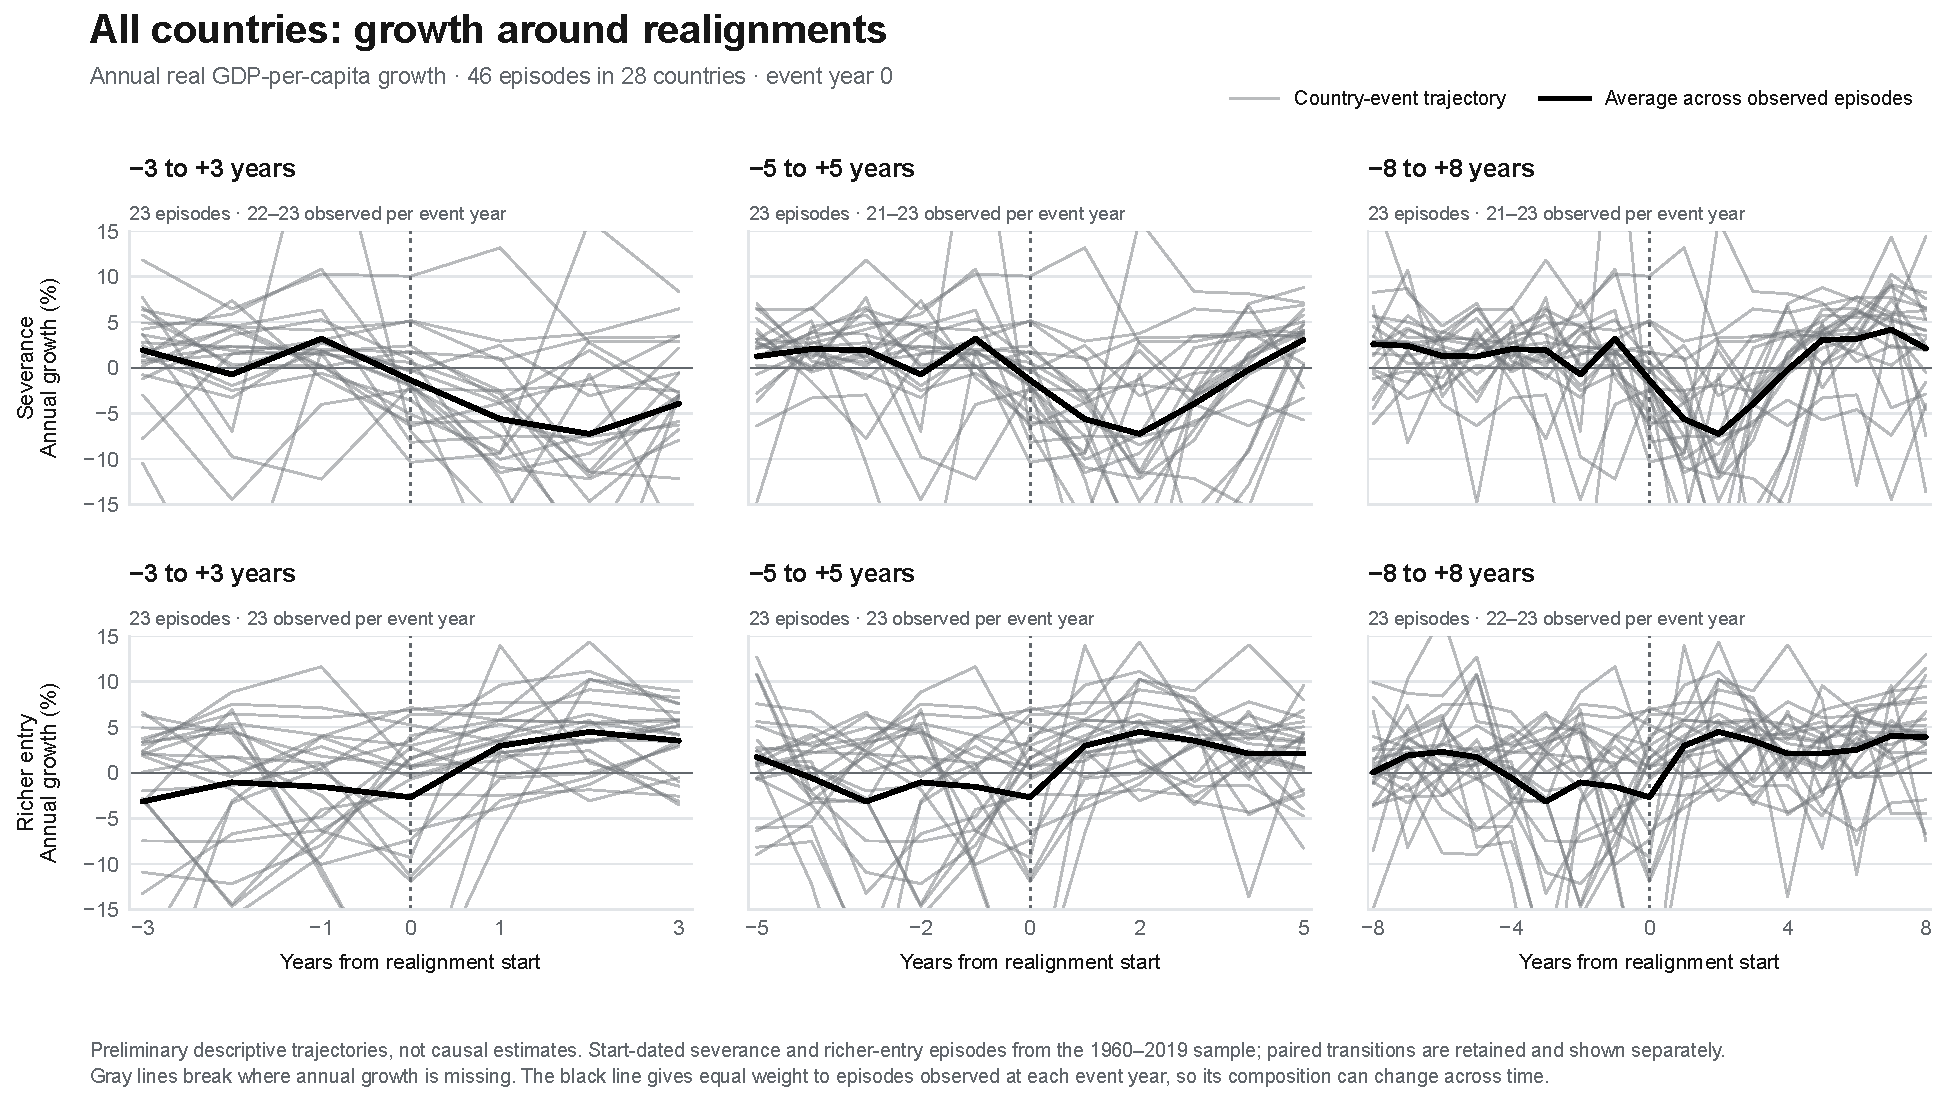
\includegraphics[width=\textwidth]{figures/event_time/all_countries_event_time_preliminary.pdf}
\caption{Annual real GDP-per-capita growth around 46 realignment episodes in 28 countries, 1960--2019. Preliminary event-time profiles.}
\label{fig:event_time_all}
\end{figure}

Table~\ref{tab:sensitivity} reports how the aggregate associations change under alternative interval dates and case-selection rules.

\begin{table}[H]
\centering
\begin{threeparttable}
\caption{Preliminary aggregate sensitivities by external event}
\label{tab:sensitivity}
\small
\begin{tabular}{@{}p{0.28\linewidth}p{0.15\linewidth}rrrr@{}}
\toprule
Scenario & External category & $N$ & $\bar g_5$ (\%) & $D_5$ (\%) & $A_8$ (\%) \\
\midrule
Start, current coding & No realignment & 4,335 & 2.23 & 21.1 & 14.4 \\
Start, current coding & Severance & 20 & $-3.28$ & 75.0 & 42.1 \\
Midpoint, current coding & Severance & 23 & $-0.16$ & 72.7 & 63.6 \\
End, current coding & Severance & 23 & 2.70 & 61.9 & 66.7 \\
Start, excluding open cases & Severance & 19 & $-2.59$ & 73.7 & 38.9 \\
Start, excluding systemic shifts & Severance & 5 & 2.53 & 40.0 & 25.0 \\
Start, imposed severance only & Severance & 6 & $-3.29$ & 83.3 & 33.3 \\
\midrule
Start, current coding & Richer entry & 20 & 3.43 & 35.0 & 60.0 \\
Midpoint, current coding & Richer entry & 23 & 3.74 & 8.7 & 13.0 \\
End, current coding & Richer entry & 23 & 2.75 & 17.4 & 13.6 \\
Start, excluding open cases & Richer entry & 18 & 3.68 & 33.3 & 61.1 \\
Start, excluding systemic shifts & Richer entry & 16 & 3.37 & 31.3 & 50.0 \\
\bottomrule
\end{tabular}
\begin{tablenotes}
\scriptsize
\item Note: Preliminary descriptive results. $\bar g_5$ is mean annual real GDP-per-capita growth over five complete forward years. $D_5$ and $A_8$ are five-year disruption and eight-year new acceleration-onset rates. Excluded event-years are removed rather than reassigned to no realignment. Valid outcome denominators vary with coverage.
\end{tablenotes}
\end{threeparttable}
\end{table}

Severance mean growth rises from $-3.28$ percent at interval starts to $+2.70$ percent at endpoints. Excluding systemic-shift episodes leaves five bare-severance observations with positive mean growth. Six imposed severances retain negative mean growth of $-3.29$ percent and an 83.3 percent disruption rate, although this subset is small and historically clustered. Richer-entry growth remains positive under all dating rules, while its acceleration-onset rate falls from 60.0 percent at starts to approximately 13 percent at midpoints and endpoints. Entry patterns therefore depend on both the outcome measure and dating convention.

\section{Expected Contribution and Remaining Work}

The preliminary evidence offers a promising empirical foundation for the project. Under start coding, severance is associated with substantially weaker subsequent growth and more frequent disruption, while entry into a richer sphere is associated with stronger growth and more frequent acceleration. The persistence of negative growth and high disruption among imposed severances further strengthens the rationale for investigating this mechanism. Pre-existing and wrong-sign outcomes identify variation that the next stage can use to establish the framework's scope conditions and refine its predictions.

The next stage will estimate the panel models, complete matched comparisons and process tracing, and measure changes in material-capability flows, including market access, capital, technology, energy prices, subsidies, and security guarantees. Open realignment judgments, unknown constitutional-amendment content, unverified post-2015 turnover, the uncoded sudden-stop component of disruption, and independent double-coding remain unresolved. Anomalous cases will stay in the data. These steps will test the necessity and sufficiency claims and clarify the direction of the observed relationships.

The completed project will contribute a transparent event taxonomy and a replicable research design linking domestic political organization, international position, and economic development. Its central empirical test is whether changes in states' material capabilities explain major economic discontinuities more effectively than nominal political transitions alone.

\printbibliography

\end{document}
